% !TeX spellcheck = en_US
\section{Background and Motivation}
\label{sec_motivation}

\subsection{A Motivating Example}
\label{subsec_motivating_example}

\begin{figure}[htbp]
	\centering
	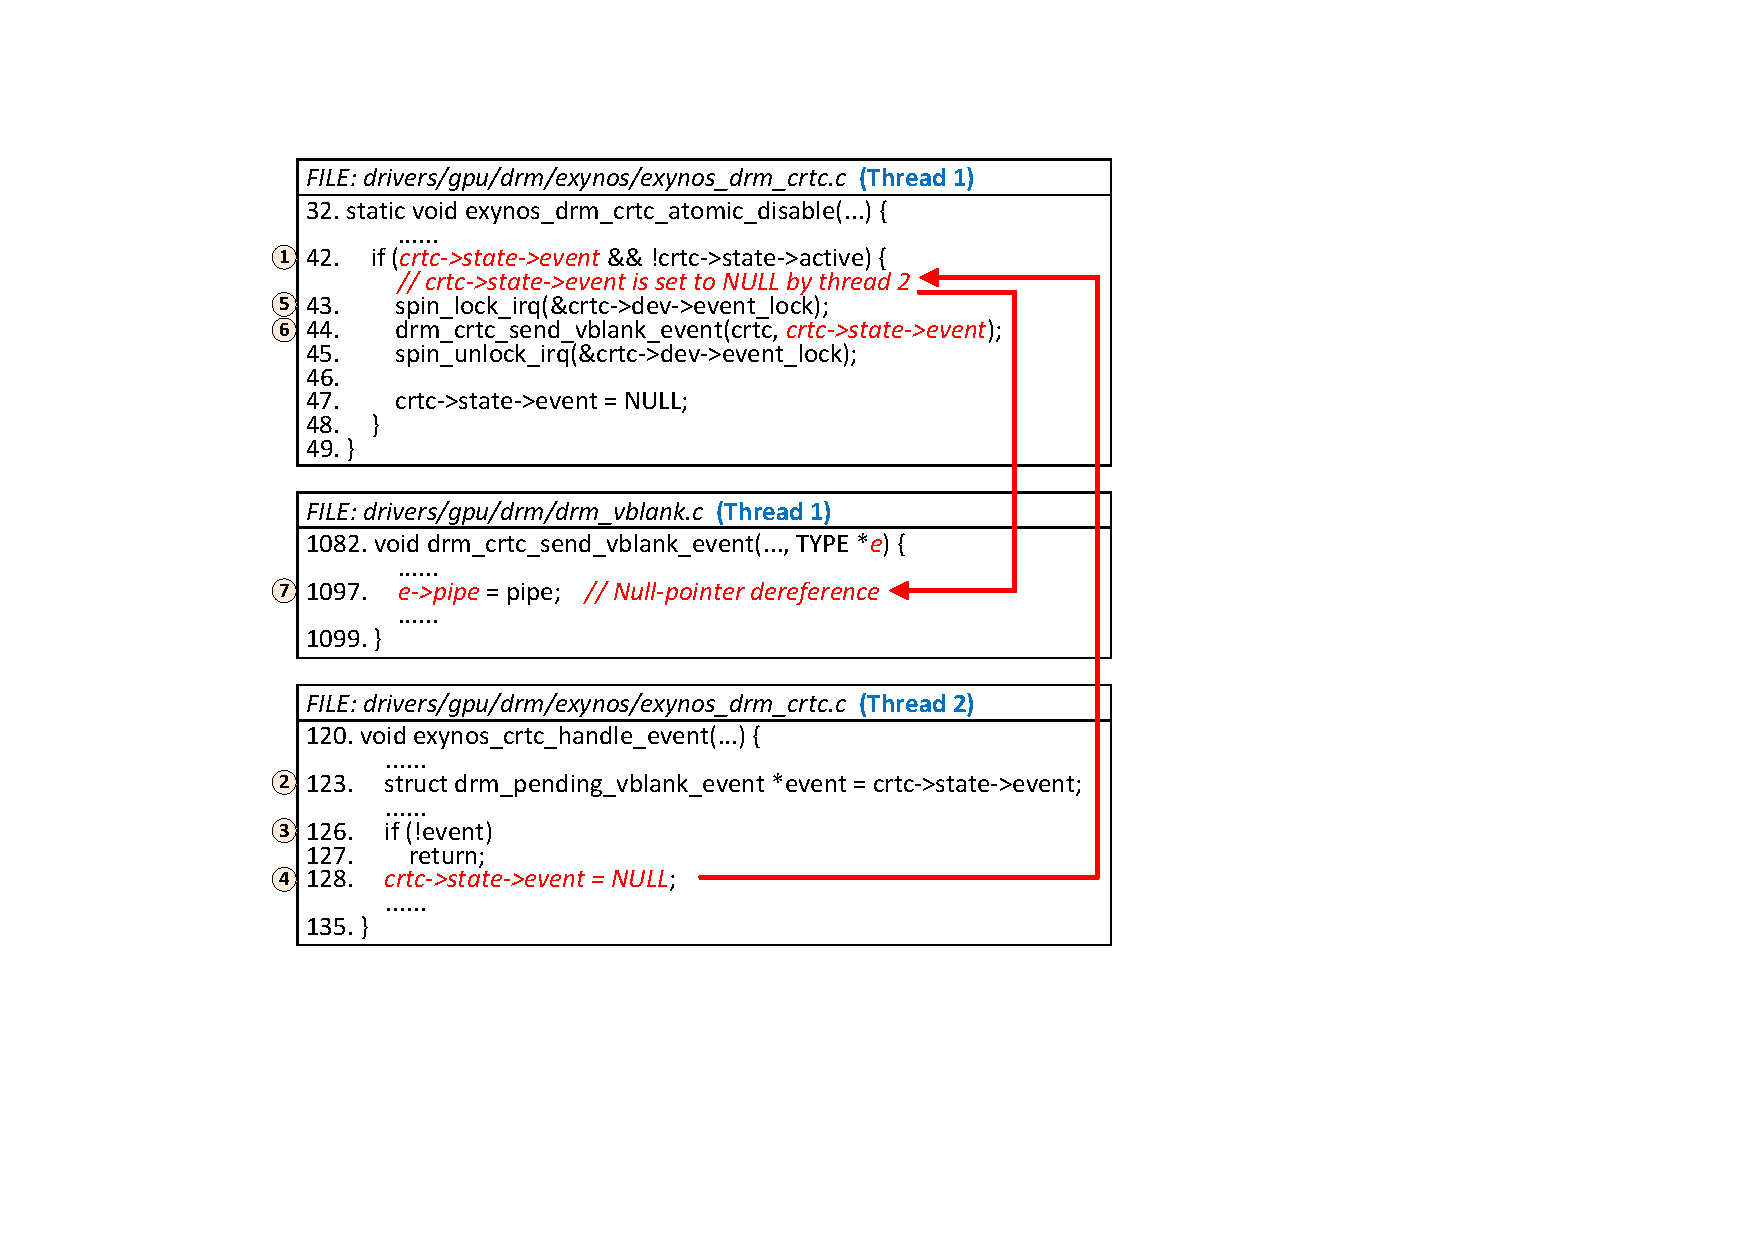
\includegraphics[width=1\linewidth]{figures/fig_demo_bug.pdf}
	\figcaption{A null-pointer dereference due to data race in Linux 6.2.}
	\label{fig_demo_bug}
\end{figure}
Figure~\ref{fig_demo_bug} shows a real null-pointer dereference caused by a 
data race in the Linux DRM driver. In the DRM driver, the functions {\tt 
exynos\_drm\_crtc\_atomic\_disable()} and {\tt exynos\_crtc\_handle\_event()} 
can execute concurrently. We exploit \textcircled{\footnotesize{n}} to 
represent the execution order of instructions and show one execution case in 
the left of Figure~\ref{fig_demo_bug}. In Thread 1, the variables {\tt 
crtc->state->event} and {\tt crtc->state->active} is checked by an if statement 
in the function {\tt exynos\_drm\_crtc\_atomic\_disable()}. After the condition 
is calculated to be true, the function {\tt exynos\_crtc\_handle\_event()} is 
executed in Thread 2. In this function, the value of {\tt crtc->state->active} 
is assigned to {\tt event} (\textcircled{\footnotesize{2}}) and then {\tt 
event} is checked in an if statement (\textcircled{\footnotesize{3}}). If it is 
not NULL, the variable {\tt crtc->state->event} is assigned with NULL 
(\textcircled{\footnotesize{4}}). Right after this assignment, the function 
{\tt drm\_crtc\_send\_vblank\_event} is called  in Thread 1 
(\textcircled{\footnotesize{6}}) with the argument {\tt crtc->state->active}, 
after acquiring the lock {\tt crtc->dev->event\_lock} 
(\textcircled{\footnotesize{5}}). In the called function, the variable {\tt 
crtc->state->event} is dereferenced through {\tt e->pipe} 
(\textcircled{\footnotesize{6}}). In this execution case, the data structure 
{\tt crtc->state->event} is first assigned with NULL and then dereferenced, and 
thus a null-pointer dereference can occur.

This bug is triggered only when {\tt crtc->state->event} is set to NULL by 
Thread 2 right after the first condition of the if statement in Thread 1 is 
calculated to be true. Such requirement is difficult to satisfy by executing 
existing test suites. In fact, this bug had existed for nearly 6 years since 
Linux 4.14 (Released in Nov. 2017), and it was fixed by us based on a report 
generated by \sys. 
 
\subsection{Challenges}
\label{subsec_challenges}
Detecting data races and estimating their harmfulness in OS kernels have three 
main challenges:

\PP{C1: Getting locking rules.} The relationship between variables and locks 
are not well documented in OS kernels, making it hard to determine whether a 
specific variable should be protected by a lock and which lock is 
required (locking rules), even for an expert developer. And thus existing 
annotation-based approaches~\cite{Boyapati:OOPSLA02, Anderson:PLDI08, 
Anderson:PLDI09, Zhou:MICRO19, Flanagan:PASTE01, Flanagan:PLDI00, 
Sadowski:PLATEAU14, ClangThreadSafety, Blackshear:OOPSLA18} are difficult to 
apply to race detection in OS kernels. Other approaches~\cite{Choi:PLDI02, 
Engler:SOSP03, Voung:FSE07, Pratikakis:PLDI06, Naik:PLDI06} employ 
lockset-based analysis to detect data races automatically, but they do not 
consider alias relations~\cite{Voung:FSE07, Engler:SOSP03} or just use 
imprecise flow-insensitive alias analysis~\cite{Choi:PLDI02, 	
Pratikakis:PLDI06, Naik:PLDI06}. However, due to the heavy use of pointers and 
data structure fields in OS code, the alias relationships between variables can 
be very complex, and thus lacking effective alias analysis can introduce many 
false locking rules.

\PP{C2: Dropping false data races.} Static analysis suffers from false 
positives. For example, each data race involves more than one code paths that 
should be able to concurrently execute. However, which code can execute 
concurrently is not well documented for an OS kernel, and it is also hard to 
determine concurrent code statically due to the complexity of OS code. Thus 
static analysis can report many false data races.

\PP{C3: Estimating harmfulness of data races.} Many data races are benign, and 
can not cause memory or logic bugs, and thus developers are unwilling to put 
effort into repairing them. To automatically detect harmful data races, most 
approaches~\cite{Narayanasamy:PLDI07, Sen:PLDI08, Kasikci:SOSP13, 
Kasikci:ASPLOS12} estimate harmfulness of data races through dynamic analysis, 
and explore thread interleavings to trigger data races to estimate their 
harmfulness. However, they suffer from low code coverage and thus can miss many 
real harmful data races.


